\documentclass[10pt,twoside,cucitura,classica,english,openany]{toptesi}

\usepackage{hyperref}
\hypersetup{%
  pdfpagemode={UseOutlines},
  bookmarksopen,
  pdfstartview={FitH},
  colorlinks,
  linkcolor={blue},
  citecolor={red},
  urlcolor={blue}
}
\usepackage[latin1]{inputenc}
\usepackage[T1]{fontenc}\usepackage{lmodern}
\usepackage{layaureo}
\usepackage{amsmath}
\usepackage{amssymb}
\usepackage{placeins}
\usepackage[titletoc]{appendix}
\usepackage[font=footnotesize]{caption}
\usepackage[font=footnotesize]{subcaption}
\usepackage[style=numeric, sorting=none, backend=biber]{biblatex}
\addbibresource{references.bib}

\bibliography{bibliography}

\ateneo{Stockholm University}
\facolta{Department of Physics}

\titolo{Search for in Mono-jet Final States with the ATLAS Experiment}

\TesiDiLaurea{Licensiate Thesis}

\CorsoDiLaureaIn{Doctoral Studies in }
\corsodilaurea{Physics}

\CandidateName{Candidate:}
\candidato{Gabriele \textsc{Bertoli}}
\AdvisorName{Advisor:}
\relatore{dott.~Christophe \textsc{Clement}}
\CoAdvisorName{Co-Supervisor}
\secondorelatore{dott.~David \textsc{Milstead}}
\sedutadilaurea{December 2015}
\sedutadilaurea{\textsc{December 12,} 2015}
\logosede{logo}

\newtheorem{osservazione}{Osservazione}
\ExtendCaptions{english}{Abstract}{Acknowledgments}

\graphicspath{{images/}}

\begin{document}\errorcontextlines=9

\numberwithin{equation}{section}

\newcommand*{\parder}[2]{\displaystyle\frac{\partial #1}{\partial #2}}
\newcommand*{\ud}{\mathrm{d}}
\newcommand*{\er}{e_{R}}
\newcommand*{\el}{e_{L}}
\newcommand*{\eplus}{e^{+}}
\newcommand*{\eminus}{e^{-}}
\newcommand*{\vect}[1]{\overrightarrow{#1}}
\newcommand*{\bra}[1]{\langle #1|}
\newcommand*{\ket}[1]{|#1\rangle}
\newcommand*{\MET}{\mbox{$E\kern-0.50em\raise0.10ex\hbox{/}_{T}$}}
\newcommand*{\met}{E_\mathrm{\, T}^\mathrm{\, miss}}
\newcommand*{\et}{E_\mathrm{\, T}}
\newcommand*{\pt}{p_\mathrm{\, T}}
\newcommand*{\ifb}{\mbox{fb$^{-1}$}}
\newcommand*{\zee}{Z \to e e}
%%% Local Variables:
%%% mode: latex
%%% TeX-master: "main"
%%% End:


\english

\cleardoublepage

% \expandafter\ifx\csname StileTrieste\endcsname\relax
\frontespizio
% \else
\paginavuota
\begin{dedica}
\end{dedica}
% \tomo \fi

\ringraziamenti

\tablespagetrue\figurespagetrue \indici

% \expandafter\ifx\csname StileTrieste\endcsname\relax \else
\begin{citazioni}
  \textit{Si sta,\\come d'autunno,\\sugli alberi,\\le foglie }

  [\textsc{G.~Ungaretti}, Soldati]
\end{citazioni}

% \fi

\chapter*{Introduction}
\label{cha:intro}
The Standard Model of particle physics is the theory used to describe the
elementary constituents of matter and their interactions. Through the years is
has been tested by many experiments and despite its success it cannot explain,
among other problems, the so called hierarchy and dark matter problems described
in \cref{cha:beyond-stand-model}. Supersymmetry is an extension of the Standard
Model that could solve these issues by introducing new particles. The lightest
of these particles, the so called neutralino (and denoted by
$\widetilde{\chi}_{\, 1}^{\, 0}$), in the context of a minimal supersymmetric
model, could be produced in squark pair production with $\squarkprod$ and,
lacking electromagnetic and strong interaction~\cite{MSSMIntro}, escape
detection. With an energy in the center of mass of $\sqrt{s} = 13$~TeV, the
\gls{lhc} could be able to produce such kind of particles, the ATLAS detector
could be able to infer their presence by the momentum unbalance they would
create. This thesis presents the result of the search for compressed
supersymmetric squark--neutralino signal with the ATLAS detector in the
3.2~$\ifb$ delivered in 2015 in an experimental signature with jets and large
missing transverse momentum in the final state.
%%% Local Variables:
%%% mode: latex
%%% TeX-master: "../search_for_DM_LED_with_ATLAS"
%%% End:


\part{Theoretical Overview}

\mainmatter

\chapter{The Standard Model of Particle Physics}
\label{cha:SM}
\section{The Standard Model}
The \emph{Standard Model} (SM) is a theoretical model which describes the
elementary constituents of matter and their interactions. Up to now, we
discovered four kind of different interactions, the \emph{electromagnetic}, the
\emph{gravitational}, the \emph{strong} and the \emph{electro-weak interaction};
excluding gravity, all of them are described by means of a \emph{quantum field
  gauge theory}.

The Standard Model is the collection of these gauge theories, it is based on the
gauge symmetry group $SU(3)_C \times SU(2)_L \times U(1)_Y$ where $SU(3)_C$ is
the symmetry group of the \emph{Quantum Chromo-Dynamics} (QCD), the ``C''
subscript stand for \emph{color charge} which is the conserved charge in the
strong interaction. The $SU(2)_L$ is the weak isotopic spin group acting on
\emph{left-handed} doublet of fermions while the $U(1)_Y$ group is the
\emph{hypercharge} symmetry group of the \emph{right-handed} fermion
singlets. Together $SU(2)_L \times U(1)_Y$ form the electro-weak symmetry group.

The Standard Model also contains and (sometimes) predicts the existence of
\emph{elementary particles} that interacts between them via the forces mentioned
above. The matter constituents are called \emph{fermions}, the interaction are
mediated by other particles called \emph{gauge bosons}. Fermions are further
categorized into \emph{quark} and \emph{leptons} and are the true fundamental
constituents of matter; the gauge bosons arise by means of symmetry property of
the Standard Model symmetry group.

The existence of all the leptons, quarks and gauge bosons is confirmed by
experimental tests. Among the bosons, the Higgs boson is peculiar because,
unlike the others, it is not associated with any interaction, instead is
postulated as a consequence of the \emph{spontaneously broken symmetry} of the
electroweak sector which is the property, responsible of giving mass to all the
elementary particles and the weak gauge bosons.

\subsection{Electro-Weak Symmetry Group}
\label{sec:electro-weak-symm}

We can now see how to find out the weak interaction symmetry group, to this end,
let us start by writing out the \emph{Hamiltonian}
\begin{equation}
  H_{weak} = \frac{4 G_F}{\sqrt{2}} J_\mu^\dagger J^\mu
\end{equation}
where
\begin{equation}
  \begin{split}
    J_\mu & \equiv J_\mu^{(+)} = \bar{\psi}_{\nu_e} \gamma_\mu \frac{1}{2} (1 -
    \gamma_5) \psi_e \equiv \bar{\nu}_{e_L}
    \gamma_\mu e_L \\
    J_\mu^\dagger & \equiv J_\mu^{(-)} = \bar{\psi}_e \gamma_\mu \frac{1}{2} (1
    - \gamma_5) \psi_{\nu_e} \equiv \bar{e}_L \gamma_\mu \nu_{e_L}
  \end{split}
\end{equation}
to easy the notation, let us write
\begin{equation}
  \chi_L =
  \begin{pmatrix}
    \nu_{e_L} \\ e^-_L
  \end{pmatrix}
  \equiv
  \begin{pmatrix}
    \nu_e \\ e^-
  \end{pmatrix}
\end{equation}
and using the Pauli matrices
\begin{equation}
  \tau_\pm = \frac{1}{2}( \tau_1 \pm i \tau_2)
\end{equation}
we have
\begin{equation}
  \begin{split}
    J_\mu^{(+)} &= \bar{\chi}_L \gamma_\mu \tau_+ \chi_L \\
    J_\mu^{(-)} &= \bar{\chi}_L \gamma_\mu \tau_- \chi_L
  \end{split}
\end{equation}
by introducing a ``neutral'' current
\begin{equation}
  J_\mu^{(3)} = \bar{\chi}_L \gamma_\mu \frac{\tau_3}{2} \chi_L = \frac{1}{2} \bar{\nu}_L \gamma_\mu \nu_L - \frac{1}{2} \bar{e}_L \gamma e_L
\end{equation}
we have a ``triplet'' of currents
\begin{equation}
  \label{eq:1}
  J_\mu^i = \bar{\chi}_L \gamma_\mu \frac{\tau_i}{2} \chi_L.
\end{equation}

Now if we pick up an $SU(2)_L$ transformation
\begin{equation}
  \chi_L (x) \to \chi'_L (x) = e^{i \vec{\varepsilon} \cdotp \vec{T}} \chi_L(x) = e^{i \vec{\varepsilon} \cdotp \frac{\vec{\tau}}{2}} \chi_L(x),
\end{equation}
where $T_i = \tau_i / 2$ are the $SU(2)_L$ \emph{generators}, and think the
$\chi_L$ as the \emph{fundamental representation}, then the current triplet is a
triplet of $SU(2)_L$, the \emph{weak isotopic spin}.

The right handed fermions are singlet for the $SU(2)_{L}$, thus
\begin{equation}
  e_{R} \to e'_{R}= e_{R}.
\end{equation}
Since we are considering the global transformations, we have no interaction, so
the Lagrangian reads
\begin{equation}
  \label{eq:2}
  \mathcal{L} = \bar{e} i \gamma^{\mu} \partial_{\mu} e + \bar{\nu} i
  \gamma^{\mu} \partial_{\mu} \nu \equiv \bar{\chi_{L}} i
  \gamma \partial \chi_{L} + \bar{e}_{R} i \gamma \partial e_{R};
\end{equation}
for now we are bounded to set $m_{e} = 0$, in fact the mass term couples right
and left fermion's components and it is not $SU(2)_{L}$ invariant.  In 1973,
experiments detected events of the type
\begin{equation}
  \label{eq:3}
  \bar{\nu}_{\mu}\eminus \rightarrow \bar{\nu}_{\mu}\eminus \\
\end{equation}
\begin{equation}
  \label{eq:4}
  \begin{cases}
    \nu_{\mu} N \rightarrow \nu_{\mu} X \\
    \bar{\nu}_{\mu} N \rightarrow \bar{\nu}_{\mu} X
  \end{cases}
\end{equation}
which are evidence of a neutral current. Further investigations yielded that the
neutral weak current is predominantly $V-A$ (i.e. left-handed) but not purely
$V-A$ so the $J^{(3)}_{\mu}(x)$ current introduced above can not be used as it
involves only left handed fermions.  We know a neutral current that mixes left
and right components namely the electromagnetic current
\begin{equation}
  \label{eq:5}
  J_{\mu} \equiv e J_{\mu}^{(em)} = e \bar{\psi} \gamma_{\mu} Q \psi
\end{equation}
where $Q$ is the charge operator with eigenvalue $Q = -1$ for the electron. $Q$
is the generator of the $U(1)_{(em)}$ group. So we have an isospin triplet and
we have included the right hand components, the isospin singlet, what we want to
do, is to combine them and define the hypercharge operator
\begin{equation}
  \label{eq:6}
  Y = 2 ( Q - T_{3}) \rightarrow Q = T_{3} + \frac{Y}{2},
\end{equation}
for the current we have
\begin{equation}
  \label{eq:7}
  J_{\mu}^{(em)} = J_{\mu}^{(3)} + \frac{1}{2} J_{\mu}^{Y}
\end{equation}
where
\begin{equation}
  \label{eq:8}
  J_{\mu}^{Y} = \bar{\psi} \gamma_{\mu} Y \psi
\end{equation}
so, by analogy, the hypercharge $Y$ generates a $U(1)_{Y}$ symmetry, and, as it
is a $SU(2)_{L}$ singlet, leaves \eqref{eq:2} invariant under the
transformations
\begin{equation}
  \label{eq:9}
  \begin{split}
    \chi_{L}(x) \rightarrow \chi'_{L}(x) = e^{i \beta Y} \chi_{L}(x)
    \equiv e^{i \beta y_{L}} \chi_{L} \\
    e_{R}(x) \rightarrow e'_{R}(x) = e^{i \beta Y}e_{R}(x) \equiv e^{i \beta
      y_{R}}e_{R}.
  \end{split}
\end{equation}
We thus have incorporated the electromagnetic interactions extending the group
to $SU(2)_{L} \times U(1)_{Y}$ and instead of having a single symmetry group we
have a direct product of groups, each with his own \emph{coupling constant}, so,
in addition to $e$ we will have another coupling to be found.  Since we have a
direct product of symmetry groups, the generators of $SU(2)_{L}$, $T_{i}$, and
the generators of $U(1)_{Y}$, $Y$ commute, the commutation relations are
\begin{equation}
  \label{eq:10}
  [T_{+},T_{-}] = 2 T_{3} \quad ; \quad [T_{3},T_{\pm}] = \pm T_{\pm}
  \quad ; \quad [Y,T_{\pm}] = [Y,T_{3}] = 0,
\end{equation}
member of the same isospin triplet, have same hypercharge eigenvalue; the
relevant quantum numbers are summarized in the table ~\ref{tab:hyper}.
\begin{table}[htb]
  \renewcommand{\arraystretch}{1.25}
  \centering
  \begin{tabular}{l c c c c}
    \hline
    {\bf Lepton} & $T$ & $T^{(3)}$ & $Q$ & $Y$ \\ \hline\hline
    $\nu_{e}$ & $\frac{1}{2}$ & $ \phantom{-}\frac{1}{2}$ & 0 & -1 \\
    $e_{L}^{-}$ & $\frac{1}{2}$ & $-\frac{1}{2}$ & -1 & -1 \\
    \\
    $e_{R}^{+}$ & 0 & $\phantom{-}0$ & -1 & -2 \\ \hline
  \end{tabular} \quad
  \begin{tabular}{l c c c c}
    \hline
    {\bf Quark} & $T$ & $T^{(3)}$ & $Q$ & $Y$ \\ \hline\hline
    $u_{L}$ & $\frac{1}{2}$ & $\phantom{-}\frac{1}{2}$ & $\phantom{-}\frac{2}{3}$ &
                                                                                    $\phantom{-}\frac{1}{3}$ \\
    $d_{L}$ & $\frac{1}{2}$ & $-\frac{1}{2}$ & $-\frac{1}{2}$ &
                                                                $\phantom{-}\frac{1}{3}$ \\
    $u_{R}$ & 0 & $\phantom{-}0$ & $\phantom{-}\frac{2}{3}$ & $\phantom{-}\frac{4}{3}$ \\
    $d_{R}$ & 0 & $\phantom{-}0$  $$ & $-\frac{1}{3}$ & $-\frac{2}{3}$ \\ \hline


  \end{tabular}
  \caption{Weak Isospin and Hypercharge Quantum Numbers of Leptons and Quarks}
  \label{tab:hyper}
\end{table}

\subsection{Electro-Weak Interactions}
\label{sec:electro-weak-inter}
As stated before, interactions are mediated by a gauge boson, we now want to
find out those for the electroweak interaction, to this end let us consider
\emph{local} gauge transformations
\begin{equation}
  \label{eq:11}
  \begin{split}
    \chi_{L} \rightarrow \chi'_{L} &= e^{i \vec\epsilon(x) \cdot \vec T
      + i \beta(x) Y} \chi_{L} \\
    \psi_{R} \to \psi'_{R} &= e^{i \beta(x) Y} \psi_{R},
  \end{split}
\end{equation}
introducing four gauge bosons,
$W_{\mu}^{(1)}, W_{\mu}^{(2)}, W_{\mu}^{(3)}, B_{\mu}$ (same as the number of
generators) and the \emph{covariant derivative}
\begin{equation}
  \label{eq:12}
  \begin{split}
    D_{\mu} \chi_{L} &= (\partial_{\mu} + i g \frac{\vec \tau}{2} \cdot
    \overrightarrow{W}_{\mu}(x) + i \frac{g'}{2} y_{L} B_{\mu}(x)) \chi_{L}
    \\
    &= (\partial_{\mu} + i g \frac{\vec \tau}{2}
    \cdot \overrightarrow{W}_{\mu}(x) - i \frac{g'}{2} B_{\mu}(x)) \chi_{L} \\
    D_{\mu} \psi_{R} &= (\partial_{\mu} + i \frac{g'}{2} y_{R} B_{\mu}(x))
    \psi_{R} \\
    &= (\partial_{\mu} - i \frac{g'}{2} B_{\mu}(x)) e_{R}
  \end{split}
\end{equation}
the Lagrangian \eqref{eq:2} reads
\begin{equation}
  \label{eq:13}
  \begin{split}
    \mathcal{L} &= \bar{\chi}_{L} i \gamma \partial \chi_{L} + \bar{e}_{R} i
    \gamma \partial e_{R} - g \bar{\chi}_{L} \gamma^{\mu} \frac{\vec{\tau}}{2}
    \chi_{L} \overrightarrow{W}_{\mu} + \frac{g'}{2} (\bar{\chi}_{L}
    \gamma^{\mu} \chi_{L} + 2 \bar{e}_{R} \gamma^{\mu} e_{R}) B_{\mu} \\
    &- \frac{1}{4} \overrightarrow{W}_{\mu\nu} \overrightarrow{W}^{\mu\nu} -
    \frac{1}{4} B_{\mu\nu}B^{\mu\nu}
  \end{split}
\end{equation}
where
\begin{equation}
  \label{eq:14}
  \begin{split}
    \overrightarrow{W}_{\mu\nu} &= \partial_{\mu} \overrightarrow{W}_{\nu}
    - \partial_{\nu} \overrightarrow{W}_{\nu}
    - g \overrightarrow{W}_{\mu} \times \overrightarrow{W}_{\nu} \\
    B_{\mu\nu} &= \partial_{\mu} B_{\nu} - \partial_{\nu} B_{\nu}
  \end{split}
\end{equation}
are the kinetic plus non abelian interaction term for the $SU(2)_{L}$ symmetry
(first equation) and the kinetic term for the abelian symmetry group
$U(1)_{Y}$. We can now split the Lagrangian terms to find out the field of the
vector bosons coupled to the charged current and to the neutral current.

\paragraph{Charged Currents Interaction}
\label{sec:charg-curr-inter}
Let us consider the term
\begin{equation}
  \label{eq:15}
  \mathcal{L}_{int}^{ew} = - g \bar{\chi}_{L} \gamma_{\mu}
  \frac{\vect{\tau}}{2} \chi_{L} \vect{W}_{\mu} + \frac{g'}{2}
  \bar{\chi}_{L} \gamma_{\mu} \chi_{L} B^{\mu} + g' \bar{e_{R}}
  \gamma_{\mu} e_{R} B^{\mu}
\end{equation}
defining
\begin{equation}
  \label{eq:16}
  W^{\pm}_{\mu} = \frac{1}{\sqrt{2}} W^{(1)} \mp i W^{(2)}
\end{equation}
we can write
\begin{equation}
  \label{eq:17}
  \mathcal{L}^{CC} = - \frac{g}{\sqrt{2}} (J^{(+)}_{\mu} W^{- \mu} +
  J^{(-)}_{\mu} W^{+ \mu})
\end{equation}
and recognize two charged vector bosons with coupling given by ``$g$''.

\paragraph{Neutral Current Interaction}
\label{sec:neutr-curr-inter}
The relevant term left to consider for what concerns the electroweak currents is
\begin{equation}
  \label{eq:18}
  \mathcal{L}^{NC} = -g J_{\mu}^{(3)} W^{(3) \mu} - \frac{g'}{2}
  J_{\mu}^{Y} B^{\mu},
\end{equation}
the electromagnetic interaction, $-i e J^{(em) \mu} A_{\mu}$, is embedded in
this expression as will became clear considering the \emph{spontaneously broken
  symmetry} phenomena, for now, is sufficient to define
\begin{equation}
  \label{eq:19}
  \begin{split}
    W^{(3)}_{\mu} &= \phantom{-} \cos \theta_{w} Z_{\mu} + \sin \theta_{w}
    A_{\mu}
    \\
    B^{\phantom{(3)}}_{\mu} &= - \sin \theta_{w} Z_{\mu} + \cos \theta_{w}
    A_{\mu}
  \end{split}
\end{equation}
and invert to get
\begin{equation}
  \label{eq:20}
  \begin{split}
    A_{\mu} &= \sin \theta_{w} W_{\mu}^{(3)} + \cos \theta_{w} B_{\mu}
    \\
    Z_{\mu} &= \cos \theta_{w} W_{\mu}^{(3)} - \sin \theta_{w} B_{\mu}
  \end{split}
\end{equation}
where $\theta_{w}$ is the electroweak \emph{mixing angle}. Plugging this into
\eqref{eq:18} and rearranging terms
\begin{equation}
  \label{eq:21}
  \begin{split}
    \mathcal{L}^{NC} &= -[(g \sin \theta_{w} J_{\mu}^{(3)} +
    \frac{g'}{2} \cos \theta_{w} J_{\mu}^{Y} ) A^{\mu} \\
    &\phantom{=} + \phantom{[}(g\cos \theta_{w} J_{\mu}^{(3)} - \frac{g'}{2}
    \sin \theta_{w} J_{\mu}^{Y}) Z^{\mu}]
  \end{split}
\end{equation}
since $A^{\mu}$ is the photon field, the first parenthesis must be identified
with the electromagnetic current, thus
\begin{equation}
  \label{eq:22}
  -(g \sin \theta_{w} J_{\mu}^{(3)} + \frac{g'}{2} \cos
  \theta_{w} J_{\mu}^{Y} ) A^{\mu} = - e J_{\mu}^{(em)} A^{\mu}
  \equiv - e ( J_{\mu}^{(3)} + \frac{J_{\mu}^{Y}}{2} ) A^{\mu}
\end{equation}
from which we get the relation
\begin{equation}
  \label{eq:23}
  g \sin \theta_{w} = g' \cos \theta_{w} = e
\end{equation}
and so we can rewrite \eqref{eq:18},
\begin{equation}
  \label{eq:24}
  \mathcal{L}^{NC} = - \frac{g}{\cos \theta_{w}} [J_{\mu}^{(3)} - \sin^{2} \theta_{w}
  J_{\mu}^{(em)}] Z^{\mu}
\end{equation}
so that $Z^{\mu}$ can be identified with the field for the neutral vector boson.

%%% Local Variables:
%%% mode: latex
%%% TeX-master: "../search_for_DM_LED_with_ATLAS"
%%% End:


\section{The hierarchy problem and naturalness}
\label{sec:hier-probl-natur}
The \emph{naturalness criterion} states that one such [dimensionless and
measured in units of the cut-off] parameter is allowed to be much smaller than
unity only if setting it to zero increases the symmetry of the theory. If this
does not happen, the theory is unnatural\cite{thooft:gauge}.

There are two important concepts in physics that enter in the formulation of the
naturalness principle, symmetries and effective field
theories. \emph{Symmetries} are closely connected to conservation laws, moreover
theory parameters that are protected by a symmetry, if smaller than the unit,
are not problematic according to the naturalness criterion. \emph{Effective
  field theories} are a sort of simplification of a more general theory that use
less parameters to describe the dynamics of particles with energies less than a
cut-off scale $\Lambda$.

Let us now consider the strength of the gravitational force, characterized by
the Newton's constant, G$_N$ and the weak force, characterized by the Fermi's
constant G$_F$, if we take the ratio of these we get:
\begin{equation}
  \label{eq:gf_gn_ratio}
  \frac{G_F \hbar^2}{G_N c^2} = 1.738 \times 10^{33}.
\end{equation}
The reason why this number is worth some attention is that theory parameters
close to the order of the unit in the SM, may be calculated in a more
fundamental theory, if any, using fundamental constants like $\pi$ or $e$ while
very big numbers may not have such a simple mathematical expression and thus may
lead to uncover new properties of the fundamental theory.

This number becomes even more interesting if we consider quantum effects.
\emph{Virtual particles} are not really particles but rather disturbances in a
field, these disturbances are off-shell ($E \neq m^2 + p^2$) and according to
the \emph{uncertainty principle}, $\Delta t \Delta E \geq \hbar / 2$, can appear
out of nothing for a short time that depends on the energy of the virtual
particle; according to quantum field theory, the vacuum is populated with such
disturbances. The Higgs field, has the property to couple with other SM
particles with a strength proportional to their mass. Now all these virtual
particles have a mass determined by the available energy $\Lambda$ and when the
Higgs field travels through space, it couples with these virtual particles and,
due to quantum corrections, its motion is affected and its invariant mass
squared gets a contribution proportional to $\Lambda$:
\begin{equation}
  \label{eq:delta_mh}
  \delta m_H^2 = k \Lambda^2 \text{, with } k = \frac{3 G_F}{4 \sqrt{2}
    \pi^2}(4m_t^2 - 2m_W^2 - m_Z^2 - m_H^2).
\end{equation}
Since $k \approx 10^{-2}$\cite{Giudice:2008bi}, the value of Higgs' mass
$m_H \sim G_F^{-1/2}$, should be close to the maximum energy scale $\Lambda$ and
if we assume this to be the Plank scale $M_{Pl} = G_N^{-1/2}$, the ration
$G_F/G_N$, should be close to the unity which contradicts
eq.~\eqref{eq:gf_gn_ratio}, this goes by the name of \emph{hierarchy's
  problem}.

The large quantum corrections in~\eqref{eq:delta_mh} are mainly due to the fact
that in the SM, there is no symmetry protecting the mass of the Higgs'
field. Supersymmetry (SUSY), among other things, is capable of solving the
hierarchy problem by canceling out the quantum corrections that bring $m_H$
close to $\Lambda$ thus restoring the naturalness of the SM.
%%% Local Variables:
%%% mode: latex
%%% TeX-master: "../search_for_DM_LED_with_ATLAS"
%%% End:



\chapter{The Monojet signature}
\label{cha:monojet-signature}

There are two possible cases that results in an energy imbalance in the
detector, the first one occurs in beyond Standard Model physics, that involves
the presence of particles that interact weakly or not at all with normal
matter. These particles are not detected thus leaving an energy imbalance in the
detector. In the second case, the decay products in the final state involve
neutrinos that are not detectable by ATLAS\@. To better understand the category
category of events, consider \cref{fig:susy_standard} that shows the decay
topology of squark pair production with a neutralino and two jets in the final
state. Using the two body decay energy and momentum relations~\cite{PDG}:
\begin{equation}
  \label{eq:93}
  E_q = \frac{M_{\, \tilde{q}}^2 - m_{\, \tilde{\chi}_{\, 1}^{\, 0}}^2 + m_q^2}{2
    M_{\, \tilde{q}}},
\end{equation}
\begin{equation}
  \label{eq:94}
  |\vec{p}_q| = |\vec{p}_{\, \tilde{\chi}_{\, 1}^{\, 0}}| = \frac{\left[ \left(
        M_{\, \tilde{q}}^2 - (m_q + m_{\, \tilde{\chi}_{\, 1}^{\, 0}})^2
      \right) \left( M_{\, \tilde{q}}^2 - (m_q - m_{\, \tilde{\chi}_{\, 1}^{\,
            0}})^2 \right) \right]^{1/2}}{2 M_{\, \tilde{q}}}
\end{equation}
where $M_{\, \tilde{q}}$ is the squark center of mass energy,
$m_{\, \tilde{\chi}_{\, 1}^{\, 0}}$ is the neutralino mass and $m_q$ is the
quark mass. Neglecting the quark mass ($m_q = 0$) we get that:
\begin{equation}
  \label{eq:95}
  E_q = \frac{M_{\, \tilde{q}}^2 - m_{\, \tilde{\chi}_{\, 1}^{\, 0}}^2}{2 M_{\,
      \tilde{q}}},
\end{equation}
\begin{equation}
  \label{eq:96}
  |\vec{p}_q| = |\vec{p}_{\, \tilde{\chi}_{\, 1}^{\, 0}}| = \frac{M_{\,
      \tilde{q}}^2 - m_{\, \tilde{\chi}_{\, 1}^{\, 0}}^2}{2 M_{\, \tilde{q}}}.
\end{equation}
The quark will hadronize in the calorimeter and give rise to a jet that can be
detected by the ATLAS detector only if $\pt > 20$~GeV. If for example the mass
of the squark is $M_{\, \tilde{q}} = 450$~GeV and the mass of the neutralino is
$m_{\, \tilde{\chi}_{\, 1}^{\, 0}} = 445$~GeV then it can be seen from
\cref{eq:96} that the quark and neutralino momenta are given by
$|\vec{p}_q|~=~|\vec{p}_{\, \tilde{\chi}_{\, 1}^{\, 0}}|~\simeq~5$~GeV. Since
the neutralino escape detection, this results in low $\met$ thus when the mass
of the neutralino approaches the mass of the quark this results in a low energy
jet and $\met$ that cannot be used to trigger and select the event by the ATLAS
detector. This means that there is no sensitivity to SUSY models with compressed
mass spectra (when the mass difference between the particles is small). This
problem applies to many channels of SUSY productions.



\cref{fig:susy_exclusion} shows this effect for the search for squark pair
production in the case of the squark decaying directly to a quark and a
neutralino through the mechanism illustrated in \cref{fig:susy_standard}. This
search uses a classical multijet + $\met$ analysis, it can be seen that there is
no sensitivity close to the diagonal (dashed line) in the region
$400~<~M_{\, \tilde{q}}~<~600$~GeV.

If an initial state radiation jet is present in the event, as depicted in
\cref{fig:susy_compressed}, the squark--squark system gets boosted in the
opposite direction thus increasing the momentum of the decay products and the
missing energy leading to a signature of a high $\pt$ jet on one side and
additional jets and $\met$ on the other side of the event.

Events with an energetic jet $\pt$ and large $\met$ in the final state
constitute a clean signature for new physics searches at hadron colliders.
Signals that can be studied with this experimental signature include the
production of WIMPS, the ADD model for large extra dimensions and SUSY\@.
\begin{figure}[!h]
  \centering
  \begin{subfigure}[t]{.48\linewidth}
    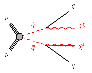
\includegraphics[width=\linewidth]{susy_standard}
    \caption{Event without initial state radiation~\cite{SUSYPub}.}
    \label{fig:susy_standard}
  \end{subfigure} \quad
  \begin{subfigure}[t]{.48\linewidth}
    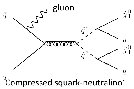
\includegraphics[width=\linewidth]{compressed}
    \caption{Event with initial state radiation~\cite{ExotPub}.}
    \label{fig:susy_compressed}
  \end{subfigure}
  \caption{Event topology of squark pair production resulting in a neutralinos
    with two jets final state with (\cref{fig:susy_compressed}) and without
    (\cref{fig:susy_standard}) initial state radiation.}
  \label{fig:motivation}
\end{figure}
\begin{figure}[!htb]
  \centering
  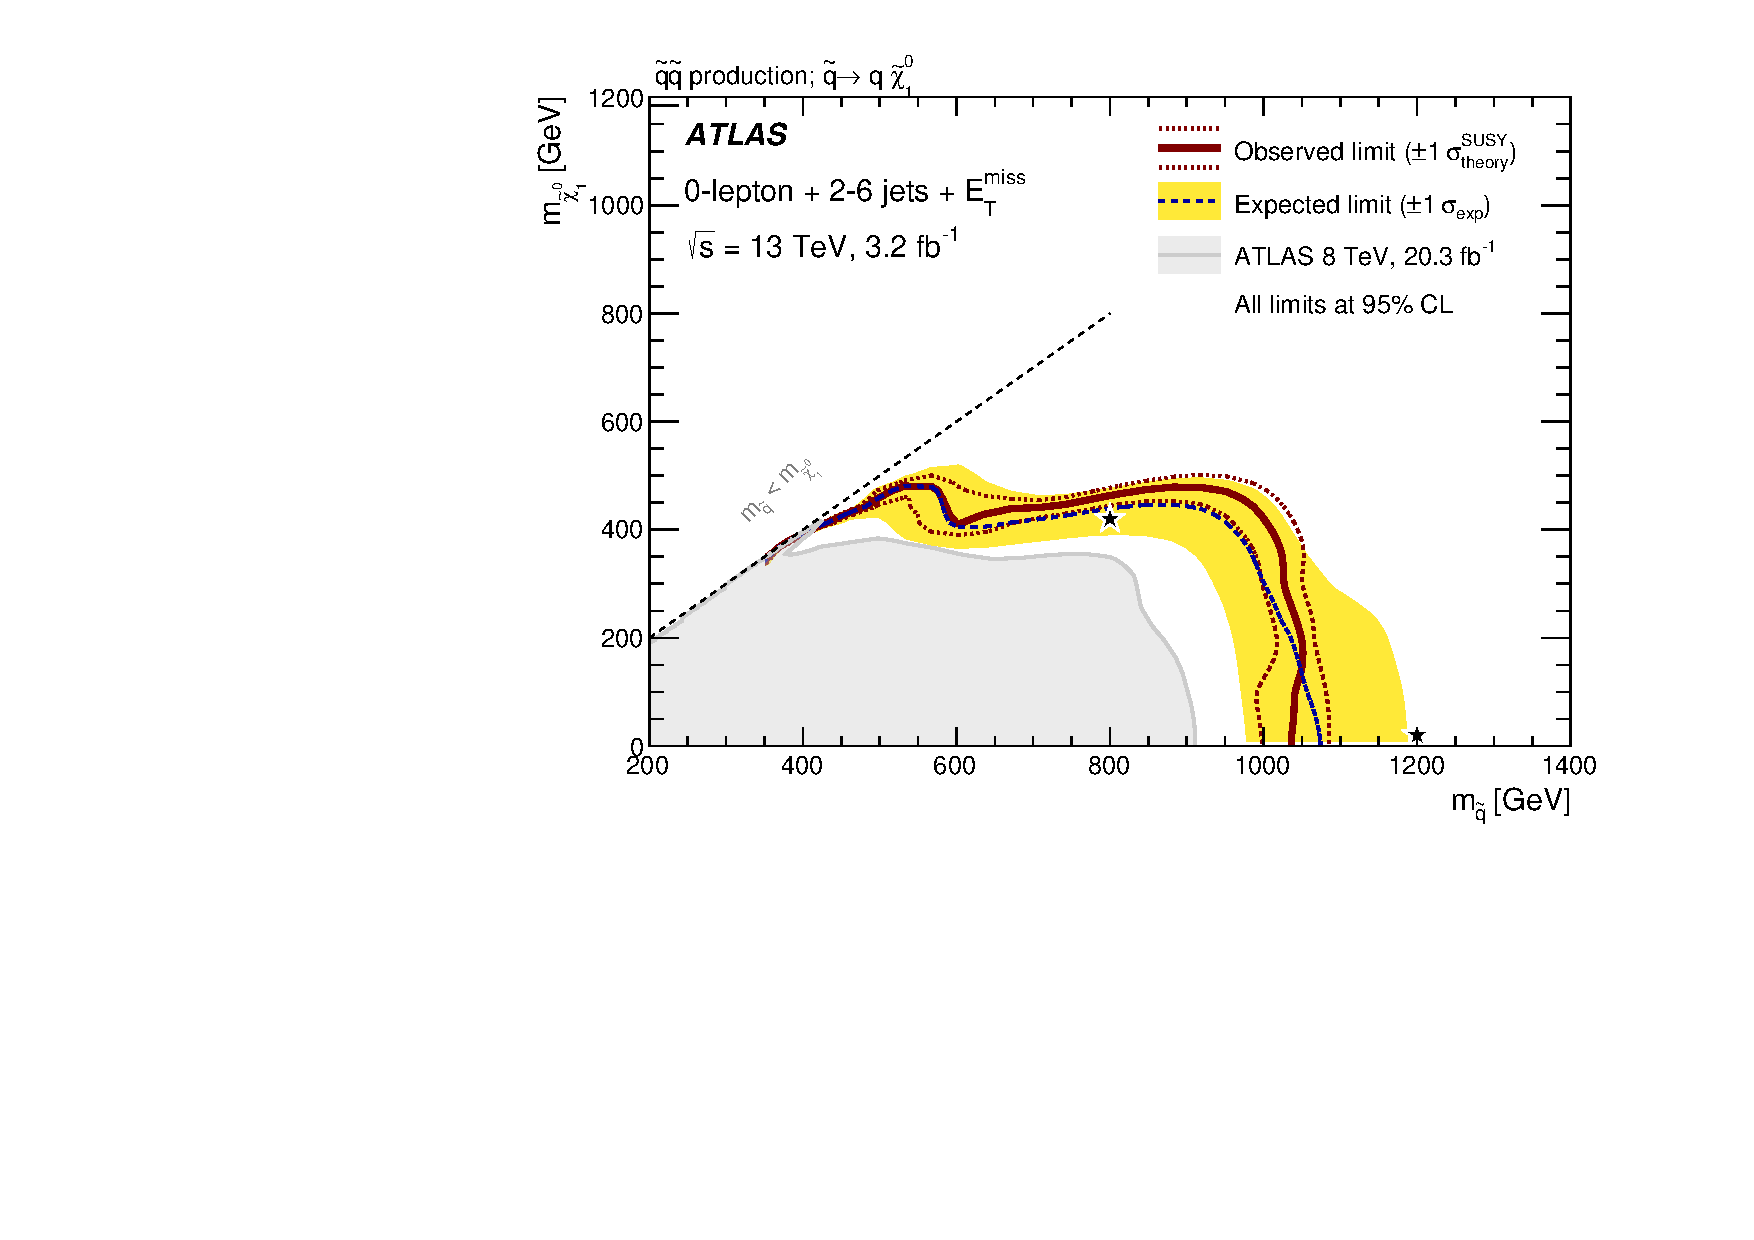
\includegraphics[width=.58\linewidth]{susy}
  \caption{Exclusion limits for direct production of squark
    pairs where the sqark decays into a quark and a neutralino. The $x$--axis
    represents the mass of the squark and the $y$--axis represents the mass of
    the lightest neutralino. The black stars represent a benchmark model as
    explained in more details in Ref.~~\cite{SUSYPub}.}
  \label{fig:susy_exclusion}
\end{figure}
%%% Local Variables:
%%% mode: latex
%%% TeX-master: "../search_for_DM_LED_with_ATLAS"
%%% End:


\section{Seraches for new physics with the monojet signature}
\label{sec:seraches-new-physics}
Events with an energetic jet \pt and large \met in the final state, constitute a
clean signature for new physics searches at hadron colliders. Signals that can
be studied with this experimental signature include the production of WIMPS,
the ADD model for large extra dimensions and SUSY.
\begin{figure}[!h]
  \centering
  \begin{subfigure}[t]{.48\linewidth}
    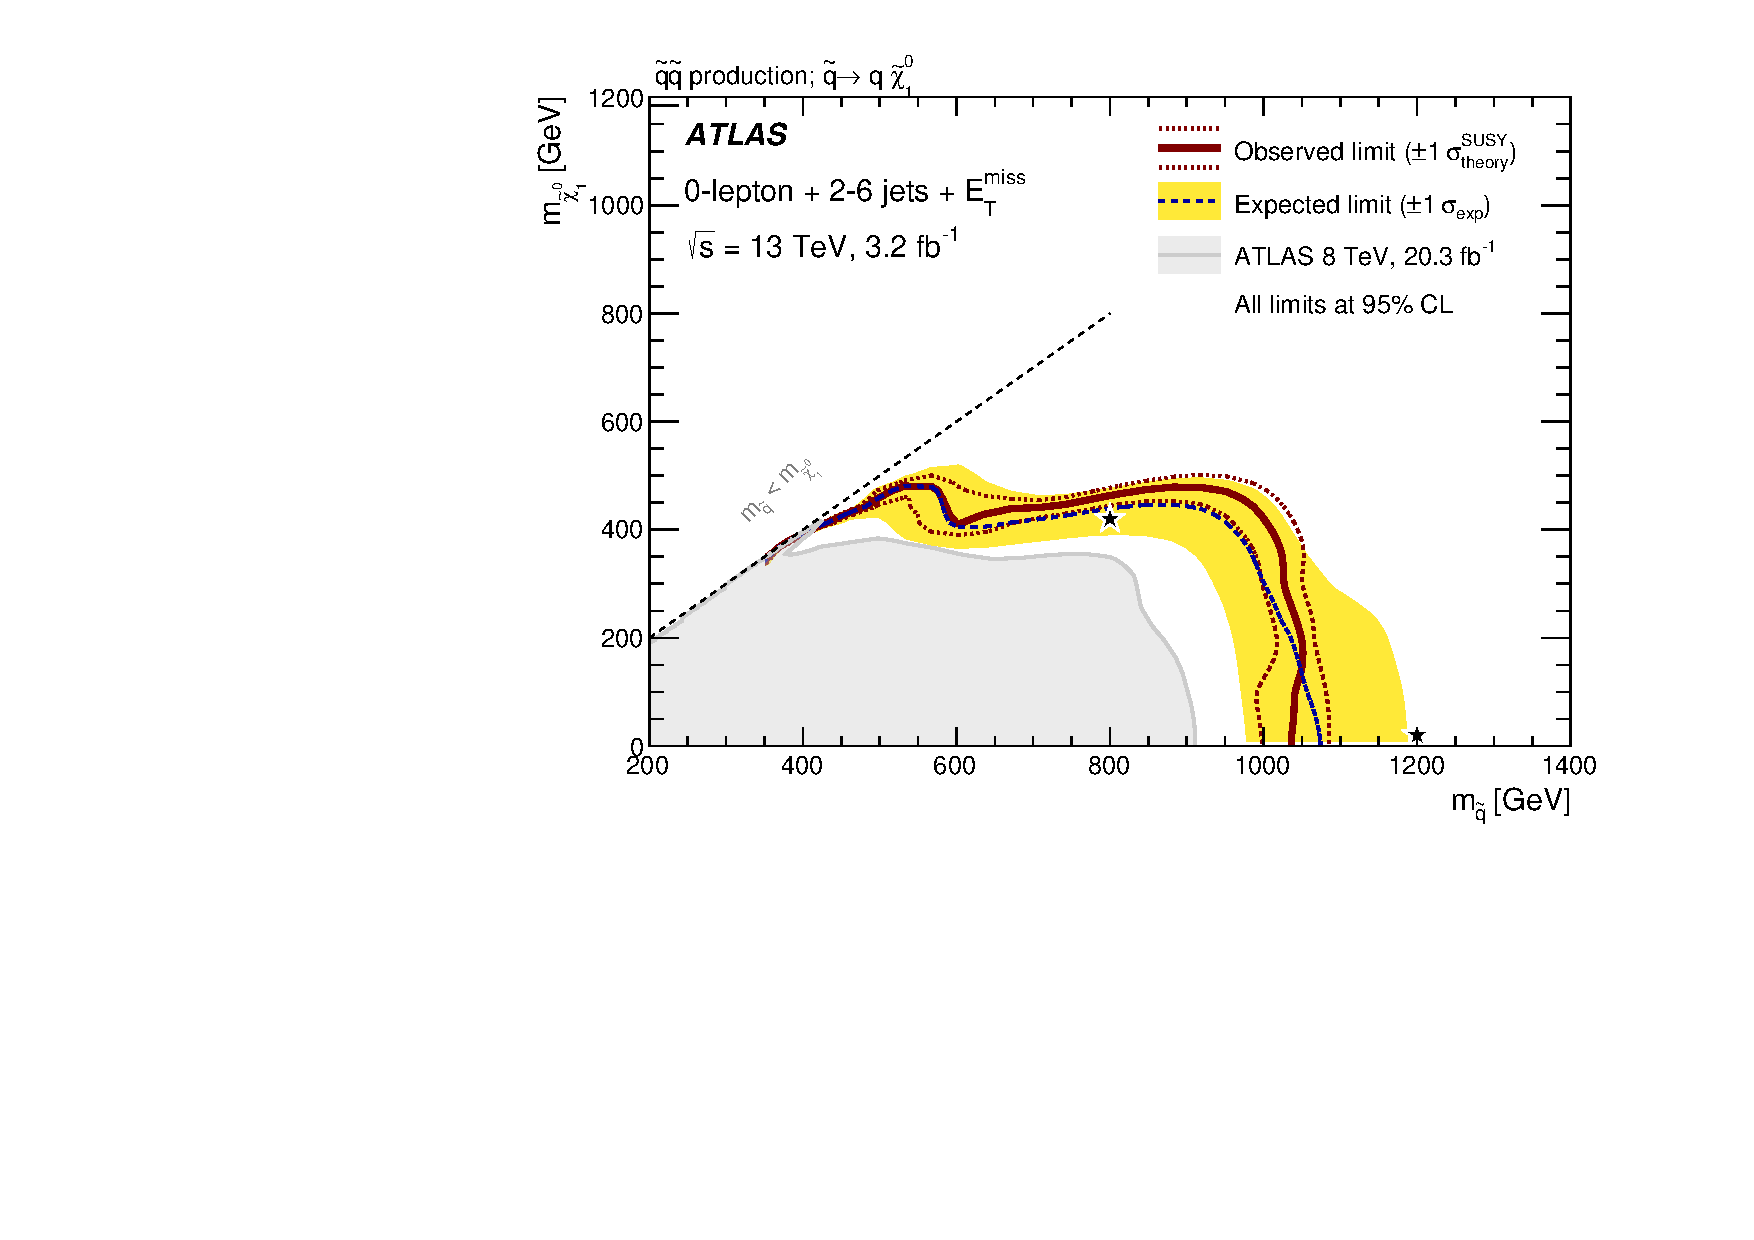
\includegraphics[width=\linewidth]{susy}
    \caption{}
    \label{fig:susy}
  \end{subfigure}
  \begin{subfigure}[t]{.48\linewidth}
    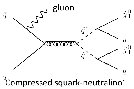
\includegraphics[width=\linewidth]{compressed}
    \caption{}
    \label{fig:compressed}
  \end{subfigure}
  \caption{}
  \label{fig:motivation}
\end{figure}
%%% Local Variables:
%%% mode: latex
%%% TeX-master: "../search_for_DM_LED_with_ATLAS"
%%% End:


\begin{appendices}
  \chapter{Some title}
\end{appendices}

\addcontentsline{toc}{chapter}{\bibname} \printbibliography
\end{document}

%%% Local Variables:
%%% mode: latex
%%% TeX-master: t
%%% End:
